%%%%%%%%%%%%%%%%%%%%%%%%%%%%%%%%%%%%%%%%%
% Classicthesis Typographic Thesis
% LaTeX Template
% Version 1.4 (1/1/16)
%
% This template has been downloaded from:
% http://www.LaTeXTemplates.com
%
% Original author:
% André Miede (http://www.miede.de) with commenting modifications by:
% Vel (vel@LaTeXTemplates.com)
%
% License:
% GNU General Public License (v2)
%
% General Tips:
% 1) Make sure to edit the classicthesis-config.file
% 2) New enumeration (A., B., C., etc in small caps): \begin{aenumerate} \end{aenumerate}
% 3) For margin notes: \marginpar or \graffito{}
% 4) Do not use bold fonts in this style, it is designed around them
% 5) Use tables as in the examples
% 6) See classicthesis-preamble.sty for useful commands
%
%%%%%%%%%%%%%%%%%%%%%%%%%%%%%%%%%%%%%%%%%

%----------------------------------------------------------------------------------------
%	PACKAGES AND OTHER DOCUMENT CONFIGURATIONS
%----------------------------------------------------------------------------------------

\documentclass[
		twosideoff,openright,titlepage,numbers=noenddot,headinclude,%1headlines,
	 	footinclude=false,cleardoublepage=empty,
		dottedtoc, % Make page numbers in the table of contents flushed right with dots leading to them
		BCOR=5mm,paper=a4,fontsize=12pt, % Binding correction, paper type and font size
		ngerman % Languages, change this to your language(s)
		]{scrreprt} 
                
% Includes the file which contains all the document configurations and packages - make sure to edit this file
%%%%%%%%%%%%%%%%%%%%%%%%%%%%%%%%%%%%%%%%%
% Classicthesis Typographic Thesis
% Configuration File
%
% This file has been downloaded from:
% http://www.LaTeXTemplates.com
%
% Original author:
% André Miede (http://www.miede.de) with extensive commenting changes by:
% Vel (vel@LaTeXTemplates.com)
%
% License:
% GNU General Public License (v2)
%
% Important note:
% The main lines to change in this file are in the DOCUMENT VARIABLES
% section, the rest of the file is for advanced configuration.
%
%%%%%%%%%%%%%%%%%%%%%%%%%%%%%%%%%%%%%%%%%

%----------------------------------------------------------------------------------------
%	CHARACTER ENCODING
%----------------------------------------------------------------------------------------

\PassOptionsToPackage{utf8}{inputenc} % Set the encoding of your files. UTF-8 is the only sensible encoding nowadays. If you can't read äöüßáéçèê∂åëæƒÏ€ then change the encoding setting in your editor, not the line below. If your editor does not support utf8 use another editor!
\usepackage{inputenc}

%----------------------------------------------------------------------------------------
%	DOCUMENT VARIABLES
%	Fill in the lines below to enter your information into the thesis template
%	Each of the commands can be cited anywhere in the thesis
%----------------------------------------------------------------------------------------

% Remove drafting to get rid of the '[ Date - classicthesis version 4.0 ]' text at the bottom of every page
\PassOptionsToPackage{eulerchapternumbers,listings,drafting, pdfspacing, subfig,beramono,eulermath,parts}{classicthesis}
% Available options: drafting parts nochapters linedheaders eulerchapternumbers beramono eulermath pdfspacing minionprospacing tocaligned dottedtoc manychapters listings floatperchapter subfig

\newcommand{\myTitle}{Asymmetrische Verschlüsselung\xspace}
\newcommand{\mySubtitle}{Einführung in die Asymmetrische Verschlüsselung\xspace}
\newcommand{\myDegree}{\xspace}
\newcommand{\myName}{Markus Brunsch\xspace}
\newcommand{\myProf}{-\xspace}
\newcommand{\myOtherProf}{Put name here\xspace}
\newcommand{\mySupervisor}{Put name here\xspace}
\newcommand{\myFaculty}{it.schule Stuttgart\xspace}
\newcommand{\myDepartment}{Put data here\xspace}
\newcommand{\myUni}{Put data here\xspace}
\newcommand{\myLocation}{Stuttgart\xspace}
\newcommand{\myTime}{Januar 2021\xspace}
\newcommand{\myVersion}{version 1.0\xspace}

%----------------------------------------------------------------------------------------
%	USEFUL COMMANDS
%----------------------------------------------------------------------------------------

\newcommand{\ie}{i.\,e.}
\newcommand{\Ie}{I.\,e.}
\newcommand{\eg}{e.\,g.}
\newcommand{\Eg}{E.\,g.} 

\newcounter{dummy} % Necessary for correct hyperlinks (to index, bib, etc.)
\providecommand{\mLyX}{L\kern-.1667em\lower.25em\hbox{Y}\kern-.125emX\@}
\newlength{\abcd} % for ab..z string length calculation

%----------------------------------------------------------------------------------------
%	PACKAGES
%----------------------------------------------------------------------------------------

\usepackage{lipsum} % Used for inserting dummy 'Lorem ipsum' text into the template

%------------------------------------------------

\PassOptionsToPackage{ngerman}{babel}  % Change this to your language(s)
% Spanish languages need extra options in order to work with this template
%\PassOptionsToPackage{spanish,es-lcroman}{babel}
\usepackage{babel}

%------------------------------------------------			

\usepackage{csquotes}
\PassOptionsToPackage{%
%backend=biber, % Instead of bibtex
backend=bibtex8,bibencoding=ascii,%
language=auto,%
style=numeric-comp,%
%style=authoryear-comp, % Author 1999, 2010
%bibstyle=authoryear,dashed=false, % dashed: substitute rep. author with ---
sorting=nyt, % name, year, title
maxbibnames=10, % default: 3, et al.
%backref=true,%
natbib=true % natbib compatibility mode (\citep and \citet still work)
}{biblatex}
\usepackage{biblatex}
 
 %------------------------------------------------

\PassOptionsToPackage{fleqn}{amsmath} % Math environments and more by the AMS 
 \usepackage{amsmath}
 
 %------------------------------------------------

\PassOptionsToPackage{T1}{fontenc} % T2A for cyrillics
\usepackage{fontenc}

%------------------------------------------------

\usepackage{textcomp} % Fix warning with missing font shapes

%------------------------------------------------

\usepackage{scrhack} % Fix warnings when using KOMA with listings package  

%------------------------------------------------

\usepackage{xspace} % To get the spacing after macros right

%------------------------------------------------

\usepackage{mparhack} % To get marginpar right

%------------------------------------------------

\usepackage{fixltx2e} % Fixes some LaTeX stuff 

%------------------------------------------------

\PassOptionsToPackage{smaller}{acronym} % Include printonlyused in the first bracket to only show acronyms used in the text
\usepackage{acronym} % Nice macros for handling all acronyms in the thesis

%\renewcommand*{\acsfont}[1]{\textssc{#1}} % For MinionPro
\renewcommand*{\aclabelfont}[1]{\acsfont{#1}}

%------------------------------------------------

\PassOptionsToPackage{pdftex}{graphicx}
\usepackage{graphicx} 

%----------------------------------------------------------------------------------------
%	FLOATS: TABLES, FIGURES AND CAPTIONS SETUP
%----------------------------------------------------------------------------------------

\usepackage{tabularx} % Better tables
\setlength{\extrarowheight}{3pt} % Increase table row height
\newcommand{\tableheadline}[1]{\multicolumn{1}{c}{\spacedlowsmallcaps{#1}}}
\newcommand{\myfloatalign}{\centering} % To be used with each float for alignment
\usepackage{caption}
\captionsetup{font=small}
\usepackage{subfig}  

%----------------------------------------------------------------------------------------
%	CODE LISTINGS SETUP
%----------------------------------------------------------------------------------------

\usepackage{listings} 
%\lstset{emph={trueIndex,root},emphstyle=\color{BlueViolet}}%\underbar} % For special keywords
\lstset{language=[LaTeX]Tex,%C++ % Specify the language(s) for listings here
morekeywords={PassOptionsToPackage,selectlanguage},
keywordstyle=\color{RoyalBlue}, % Add \bfseries for bold
basicstyle=\small\ttfamily, % Makes listings a smaller font size and a different font
%identifierstyle=\color{NavyBlue}, % Color of text inside brackets
commentstyle=\color{Green}\ttfamily, % Color of comments
stringstyle=\rmfamily, % Font type to use for strings
numbers=left, % Change left to none to remove line numbers
numberstyle=\scriptsize, % Font size of the line numbers
stepnumber=5, % Increment of line numbers
numbersep=8pt, % Distance of line numbers from code listing
showstringspaces=false, % Sets whether spaces in strings should appear underlined
breaklines=true, % Force the code to stay in the confines of the listing box
%frameround=ftff, % Uncomment for rounded frame
%frame=single, % Frame border - none/leftline/topline/bottomline/lines/single/shadowbox/L
belowcaptionskip=.75\baselineskip % Space after the "Listing #: Desciption" text and the listing box
}

%----------------------------------------------------------------------------------------
%	HYPERREFERENCES
%----------------------------------------------------------------------------------------

\PassOptionsToPackage{pdftex,hyperfootnotes=false,pdfpagelabels}{hyperref}
\usepackage{hyperref}  % backref linktocpage pagebackref
\pdfcompresslevel=9
\pdfadjustspacing=1

\hypersetup{
% Uncomment the line below to remove all links (to references, figures, tables, etc), useful for b/w printouts
%draft, 
colorlinks=true, linktocpage=true, pdfstartpage=3, pdfstartview=FitV,
% Uncomment the line below if you want to have black links (e.g. for printing black and white)
%colorlinks=false, linktocpage=false, pdfborder={0 0 0}, pdfstartpage=3, pdfstartview=FitV, 
breaklinks=true, pdfpagemode=UseNone, pageanchor=true, pdfpagemode=UseOutlines,%
plainpages=false, bookmarksnumbered, bookmarksopen=true, bookmarksopenlevel=1,%
hypertexnames=true, pdfhighlight=/O,%nesting=true,%frenchlinks,%
urlcolor=webbrown, linkcolor=RoyalBlue, citecolor=webgreen, %pagecolor=RoyalBlue,%
    %urlcolor=Black, linkcolor=Black, citecolor=Black, %pagecolor=Black,%
%------------------------------------------------
% PDF file meta-information
pdftitle={\myTitle},
pdfauthor={\textcopyright\ \myName, \myUni, \myFaculty},
pdfsubject={},
pdfkeywords={},
pdfcreator={pdfLaTeX},
pdfproducer={LaTeX with hyperref and classicthesis}
%------------------------------------------------
}

%----------------------------------------------------------------------------------------
%	AUTOREFERENCES SETUP
%	Redefines how references in text are prefaced for different 
%	languages (e.g. "Section 1.2" or "section 1.2")
%----------------------------------------------------------------------------------------

\makeatletter
\@ifpackageloaded{babel}
{
\addto\extrasamerican{
\renewcommand*{\figureautorefname}{Figure}
\renewcommand*{\tableautorefname}{Table}
\renewcommand*{\partautorefname}{Part}
\renewcommand*{\chapterautorefname}{Chapter}
\renewcommand*{\sectionautorefname}{Section}
\renewcommand*{\subsectionautorefname}{Section}
\renewcommand*{\subsubsectionautorefname}{Section}
}
\addto\extrasngerman{
\renewcommand*{\paragraphautorefname}{Absatz}
\renewcommand*{\subparagraphautorefname}{Unterabsatz}
\renewcommand*{\footnoteautorefname}{Fu\"snote}
\renewcommand*{\FancyVerbLineautorefname}{Zeile}
\renewcommand*{\theoremautorefname}{Theorem}
\renewcommand*{\appendixautorefname}{Anhang}
\renewcommand*{\equationautorefname}{Gleichung}
\renewcommand*{\itemautorefname}{Punkt}
}
\providecommand{\subfigureautorefname}{\figureautorefname} % Fix to getting autorefs for subfigures right
}{\relax}
\makeatother

%----------------------------------------------------------------------------------------

\usepackage{classicthesis} 

%----------------------------------------------------------------------------------------
%	CHANGING TEXT AREA 
%----------------------------------------------------------------------------------------

%\linespread{1.05} % a bit more for Palatino
%\areaset[current]{312pt}{761pt} % 686 (factor 2.2) + 33 head + 42 head \the\footskip
%\setlength{\marginparwidth}{7em}%
%\setlength{\marginparsep}{2em}%

%----------------------------------------------------------------------------------------
%	USING DIFFERENT FONTS
%----------------------------------------------------------------------------------------

%\usepackage[oldstylenums]{kpfonts} % oldstyle notextcomp
%\usepackage[osf]{libertine}
%\usepackage[light,condensed,math]{iwona}
%\renewcommand{\sfdefault}{iwona}
%\usepackage{lmodern} % <-- no osf support :-(
%\usepackage{cfr-lm} % 
%\usepackage[urw-garamond]{mathdesign} <-- no osf support :-(
%\usepackage[default,osfigures]{opensans} % scale=0.95 
%\usepackage[sfdefault]{FiraSans}

\addbibresource{Bibliography.bib} % The file housing your bibliography
%\addbibresource[label=ownpubs]{Self_Publications.bib} % Uncomment for optional self-publications

%\hyphenation{Put special hyphenation here}

\begin{document}

\frenchspacing % Reduces space after periods to make text more compact

\raggedbottom % Makes all pages the height of the text on that page

\selectlanguage{ngerman} % Select your default language - e.g. american or ngerman

%\renewcommand*{\bibname}{new name} % Uncomment to change the name of the bibliography
%\setbibpreamble{} % Uncomment to include a preamble to the bibliography - some text before the reference list starts

\pagenumbering{arabic} % Roman page numbering prior to the start of the thesis content (i, ii, iii, etc)

\pagestyle{plain} % Suppress headers for the pre-content pages

%----------------------------------------------------------------------------------------
%	PRE-CONTENT THESIS PAGES
%----------------------------------------------------------------------------------------

% Title Page

\begin{titlepage}

\begin{addmargin}[-1cm]{-3cm}
\begin{center}
\large

\hfill
\vfill

\begingroup
\color{Maroon}\spacedallcaps{\myTitle} \\ \bigskip % Thesis title
\endgroup

\spacedlowsmallcaps{\myName} % Your name

\vfill


\includegraphics[width=6cm]{gfx/TFZsuperellipse_bw} \\ \medskip % Picture

\mySubtitle \\ \medskip % Thesis subtitle
%\myDegree \\
%\myDepartment \\
%\myFaculty \\
%\myUni \\ \bigskip

\myTime\ -- \myVersion % Time and version

\vfill

\end{center}
\end{addmargin}

\end{titlepage} % Main title page

%% Back of the title page

\thispagestyle{empty}

\hfill

\vfill

\noindent\myName: \textit{\myTitle,} \mySubtitle, %\myDegree, 
\textcopyright\ \myTime

% You may wish to do something with the back of the title page, such as including your supervisors, location or time frame of the work. Below is an example of doing so although you may want to tweak it to your liking.

%\bigskip

%\noindent\spacedlowsmallcaps{Supervisors}: \\
%\myProf \\
%\myOtherProf \\ 
%\mySupervisor

%\medskip \\

%\noindent\spacedlowsmallcaps{Location}: \\
%\myLocation

%\medskip \\

%\noindent\spacedlowsmallcaps{Time Frame}: \\
%\myTime
 % Back of the title page

%\cleardoublepage% Dedication

\thispagestyle{empty}
\refstepcounter{dummy}

\pdfbookmark[1]{Dedication}{Dedication} % Bookmark name visible in a PDF viewer

\vspace*{3cm}

\begin{center}
\emph{Ohana} means family. \\
Family means nobody gets left behind, or forgotten. \\ \medskip
--- Lilo \& Stitch    
\end{center}

\medskip

\begin{center}
Dedicated to the loving memory of Rudolf Miede. \\ \smallskip
1939\,--\,2005
\end{center} % Dedication page

%\cleardoublepage\include{FrontBackMatter/Foreword} % Uncomment and create a Foreword.tex to include a foreword

%\cleardoublepage% Abstract

%\renewcommand{\abstractname}{Abstract} % Uncomment to change the name of the abstract

\pdfbookmark[1]{Abstract}{Abstract} % Bookmark name visible in a PDF viewer

\begingroup
\let\clearpage\relax
\let\cleardoublepage\relax
\let\cleardoublepage\relax

\chapter*{Abstract}
Short summary of the contents\dots a great guide by 
Kent Beck how to write good abstracts can be found here:  
\begin{center}
\url{https://plg.uwaterloo.ca/~migod/research/beckOOPSLA.html}
\end{center}

\endgroup			

\vfill % Abstract page

\cleardoublepage% Publications - a page listing research articles written using content in the thesis

\pdfbookmark[1]{Publications}{Publications} % Bookmark name visible in a PDF viewer

\chapter*{Publications} % Publications page text

Some ideas and figures have appeared previously in the following publications:\\

\noindent Put your publications from the thesis here. The packages \texttt{multibib} or \texttt{bibtopic} etc. can be used to handle multiple different bibliographies in your document.

%\begin{refsection}[ownpubs]
%    \small
%    \nocite{*} % is local to to the enclosing refsection
%    \printbibliography[heading=none]
%\end{refsection}

%\emph{Attention}: This requires a separate run of \texttt{bibtex} for your \texttt{refsection}, \eg, \texttt{ClassicThesis1-blx} for this file. You might also use \texttt{biber} as the backend for \texttt{biblatex}. See also \url{http://tex.stackexchange.com/questions/128196/problem-with-refsection}. % Publications from the thesis page

%\cleardoublepage% Acknowledgements

\pdfbookmark[1]{Acknowledgements}{Acknowledgements} % Bookmark name visible in a PDF viewer

\begin{flushright}{\slshape    
We have seen that computer programming is an art, \\ 
because it applies accumulated knowledge to the world, \\ 
because it requires skill and ingenuity, and especially \\
because it produces objects of beauty.} \\ \medskip
--- \defcitealias{knuth:1974}{Donald E. Knuth}\citetalias{knuth:1974} \citep{knuth:1974}
\end{flushright}

\bigskip

%----------------------------------------------------------------------------------------

\begingroup

\let\clearpage\relax
\let\cleardoublepage\relax
\let\cleardoublepage\relax

\chapter*{Acknowledgements}

\noindent Put your acknowledgements here.\\

\noindent Many thanks to everybody who already sent me a postcard!\\

\noindent Regarding the typography and other help, many thanks go to Marco Kuhlmann, Philipp Lehman, Lothar Schlesier, Jim Young, Lorenzo Pantieri and Enrico Gregorio\footnote{Members of GuIT (Gruppo Italiano Utilizzatori di \TeX\ e \LaTeX )}, J\"org Sommer, Joachim K\"ostler, Daniel Gottschlag, Denis Aydin, Paride Legovini, Steffen Prochnow, Nicolas Repp, Hinrich Harms, Roland Winkler, and the whole \LaTeX-community for support, ideas and some great software.

\bigskip

\noindent\emph{Regarding \mLyX}: The \mLyX\ port was initially done by
\emph{Nicholas Mariette} in March 2009 and continued by
\emph{Ivo Pletikosi\'c} in 2011. Thank you very much for your work and the contributions to the original style.

\endgroup % Acknowledgements page

\pagestyle{scrheadings} % Show chapter titles as headings

\cleardoublepage% Table of Contents - List of Tables/Figures/Listings and Acronyms

\refstepcounter{dummy}

\pdfbookmark[1]{\contentsname}{tableofcontents} % Bookmark name visible in a PDF viewer

\setcounter{tocdepth}{2} % Depth of sections to include in the table of contents - currently up to subsections

\setcounter{secnumdepth}{3} % Depth of sections to number in the text itself - currently up to subsubsections

\manualmark
\markboth{\spacedlowsmallcaps{\contentsname}}{\spacedlowsmallcaps{\contentsname}}
\tableofcontents 
\automark[section]{chapter}
\renewcommand{\chaptermark}[1]{\markboth{\spacedlowsmallcaps{#1}}{\spacedlowsmallcaps{#1}}}
\renewcommand{\sectionmark}[1]{\markright{\thesection\enspace\spacedlowsmallcaps{#1}}}

\clearpage

\begingroup 
\let\clearpage\relax
\let\cleardoublepage\relax
\let\cleardoublepage\relax

%----------------------------------------------------------------------------------------
%	List of Figures
%----------------------------------------------------------------------------------------

\refstepcounter{dummy}
%\addcontentsline{toc}{chapter}{\listfigurename} % Uncomment if you would like the list of figures to appear in the table of contents
\pdfbookmark[1]{\listfigurename}{lof} % Bookmark name visible in a PDF viewer

\listoffigures

\vspace{8ex}
\newpage

%----------------------------------------------------------------------------------------
%	List of Tables
%----------------------------------------------------------------------------------------

\refstepcounter{dummy}
%\addcontentsline{toc}{chapter}{\listtablename} % Uncomment if you would like the list of tables to appear in the table of contents
\pdfbookmark[1]{\listtablename}{lot} % Bookmark name visible in a PDF viewer

\listoftables
        
\vspace{8ex}
\newpage
    
%----------------------------------------------------------------------------------------
%	List of Listings
%---------------------------------------------------------------------------------------- 

\refstepcounter{dummy}
%\addcontentsline{toc}{chapter}{\lstlistlistingname} % Uncomment if you would like the list of listings to appear in the table of contents
\pdfbookmark[1]{\lstlistlistingname}{lol} % Bookmark name visible in a PDF viewer

\lstlistoflistings 

\vspace{8ex}
\newpage
       
%----------------------------------------------------------------------------------------
%	Acronyms
%----------------------------------------------------------------------------------------

\refstepcounter{dummy}
%\addcontentsline{toc}{chapter}{Acronyms} % Uncomment if you would like the acronyms to appear in the table of contents
\pdfbookmark[1]{Acronyms}{acronyms} % Bookmark name visible in a PDF viewer

\markboth{\spacedlowsmallcaps{Acronyms}}{\spacedlowsmallcaps{Acronyms}}

\chapter*{Acronyms}

\begin{acronym}[UML]
\acro{DRY}{Don't Repeat Yourself}
\acro{API}{Application Programming Interface}
\acro{UML}{Unified Modeling Language}
\end{acronym}  
                   
\endgroup % Contents, list of figures/tables/listings and acronyms

\cleardoublepage

%\pagenumbering{arabic} % Arabic page numbering for thesis content (1, 2, 3, etc)
%\setcounter{page}{90} % Uncomment to manually start the page counter at an arbitrary value (for example if you wish to count the pre-content pages in the page count)

\cleardoublepage % Avoids problems with pdfbookmark

%----------------------------------------------------------------------------------------
%	THESIS CONTENT - CHAPTERS
%----------------------------------------------------------------------------------------

\ctparttext{You can put some informational part preamble text here. Illo principalmente su nos. Non message \emph{occidental} angloromanic da. Debitas effortio simplificate sia se, auxiliar summarios da que, se avantiate publicationes via. Pan in terra summarios, capital interlingua se que. Al via multo esser specimen, campo responder que da. Le usate medical addresses pro, europa origine sanctificate nos se.} % Text on the Part 1 page describing  the content in Part 1

\part{Einführung in die Kryptographie} % First part of the thesis

% Chapter 1

\chapter{Einführung} % Chapter title

\label{ch:introduction} % For referencing the chapter elsewhere, use \autoref{ch:introduction} 

%----------------------------------------------------------------------------------------

\section{Geschichte der Kryptographie}

%---------

\paragraph{Altertum}
\hfill\\
Erste frühe Varianten waren geheimnachrichten die versteckt Transportiert wurden.\\
So wurden beispielweise in Ägypten Sklaven die Haare abrasiert eine Nachricht eintätowiert und nachdem die Haara nachgewachsen waren zum Empfänger geschickt.
Eine weitere Variante waren kleine Löcher in Buchstabenform auf Papyrusrollen, die erst bei Gegenlicht dann sichtbar wurden.
\\ Auch in Griechenland wurde bereits 500 v.Chr. ein Verschlüsselungsstab namens Skytale\footnote{\url{https://de.wikipedia.org/wiki/Skytale}} Entwickelt mit deren Hilfe Texte verschlüsselt werden konnten.

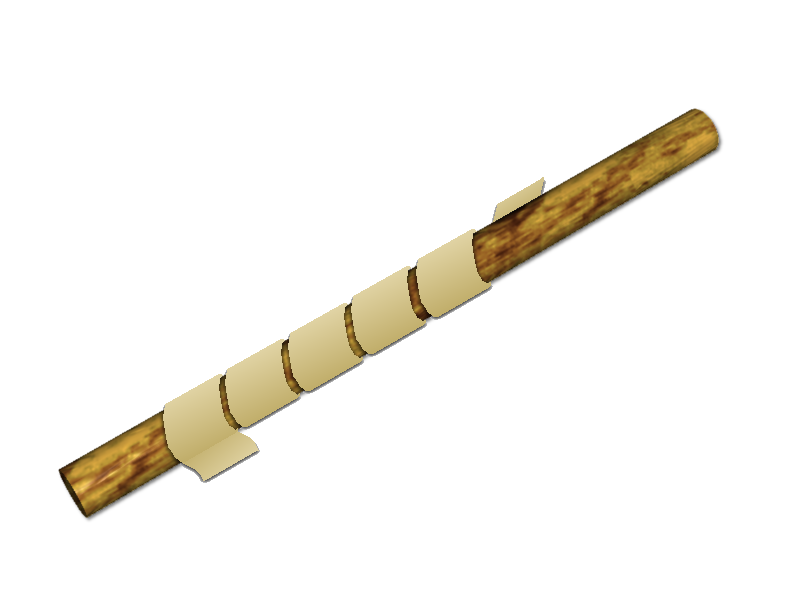
\includegraphics[width=5cm]{gfx/Skytala}% Picture
\hfill
\\ Julius Cäsar (etwa 100 v. Chr. bis 44 v. Chr.) soll die nach ihm benannte Cäsar-Chiffre \footnote{\url{https://de.wikipedia.org/wiki/Gaius_Iulius_Caesar}} genutzt haben, die jeden Buchstaben im Alphabet um einen festgelegten Wert verschiebt.
\\Auszüge aus dem Paper von \citeauthor{huetter:geschichte} ``Geschichte der Kryptographie`'\citep{huetter:geschichte}
%---------

\paragraph{Mittelalter}
\hfill\\
\citeauthor{al-kadi}Zwischen den Jahren 500 und 1400 gab es vor allem aus der arabischen Welt bedeutende Beiträge zur Kryptographie.\citep{al-kadi}
In Europa soll Karl der Große als Verschlüsselungsmethode ein unbekanntes Alphabet in verbindung mit einem Einsetzungsverfahren verwendet haben.
\newpage
%---------

\paragraph{Neuzeit}
\hfill\\
Zwischen dem 14. und 17. Jahrhundert hat die Kryptographie wie viele andere Wissentschaften einen großen Aufschwung.
Die kaum veränderten Varfahren wurden in dieser Zeit weiterentwickelt.
\\Hier eine Auflistung der Innovationen dieser Zeit
\begin{itemize}
    \item Chiffrierscheibe \footnote{Chiffrierscheibe\\\url{https://de.wikipedia.org/wiki/Chiffrierscheibe}}
    \item Voynich-Manuskript \footnote{Voynich-Manuskript\\\url{https://de.wikipedia.org/wiki/Voynich-Manuskript}}
    \item Beale-Chiffre \footnote{Beale-Chiffre\\\url{https://de.wikipedia.org/wiki/Beale-Chiffre}}
    \item Dorabella-Chiffre \footnote{Dorabella-Chiffre \\\url{https://de.wikipedia.org/wiki/Dorabella-Chiffre}}
    \item Weiterentwicklung durch Aufkommen der Telegrafie \footnote{Kerckhoffs Prinzip \\\url{https://de.wikipedia.org/wiki/Kerckhoffs_Prinzip}}
\end{itemize}

%----------------------------------------------------------------------------------------

\section{Begrifflichkeiten}

\subsection{Authentizität}
Beschreibt, dass eine Nachricht auch vom eigentlichen Absender verfasst und versendet wurde.
Dies ist weniger ein aspekt der Verschlüsselung sondern eher vergelichbar mit einer Unterschrift oder einem Siegel.
Authentizität dient dazu seine Identität zu bestätigen.
\citeauthor{richter}'s ``\emph{Verschlüsselung im Internet}'' \citep{richter}.
%----------------------------------------------------------------------------------------

\subsection{Integrität}

Integrität ist der Nachweis darüber, dass die Nachricht auf dem Übertragungsweg nicht verändert oder manupuliert wurde.
Die Integrität hängt von der Authentizität des Absenders ab, da nur mit der Grundlage des "echten" Absenders die Sinnhaftigkeit einer Integritätsprüfung überhaupt aufkommt.
Ist dies gegeben kann anhand von Digitalen Signaturen überprüft werden ob die Nachricht in einer weise verändert worden ist.
Dies geschieht dadurch, dass Digitale Signaturen von der gesammten Nachricht abhängen.
\citeauthor{richter}'s ``\emph{Verschlüsselung im Internet}'' \citep{richter}.

%----------------------------------------------------------------------------------------

\subsection{Vertraulichkeit}
Ziel ist es eine Nachricht nur für berechtigte Personen zugänglich zu machen und zu verhindern, dass dritte sich unbefugt Zugriff zu der Nachticht verschaffen können.

%----------------------------------------------------------------------------------------

\subsection{Verbindlichkeit}
Verbindlichkeit stelle eine eindeutige nicht abstreitbare Zurückverfolgbarkeit der Nachricht zum Absender her.
\citeauthor{wiki:itsec} ``\emph{Motivation und Ziele der Informationssicherheit}'' \citep{wiki:itsec} % Chapter 1

\cleardoublepage % Empty page before the start of the next part

%------------------------------------------------

\ctparttext{You can put some informational part preamble text here. Illo principalmente su nos. Non message \emph{occidental} angloromanic da. Debitas effortio simplificate sia se, auxiliar summarios da que, se avantiate publicationes via. Pan in terra summarios, capital interlingua se que. Al via multo esser specimen, campo responder que da. Le usate medical addresses pro, europa origine sanctificate nos se.} % Text on the Part 2 page describing the content in Part 2

\part{Asymmetrische Kryptographie} % Second part of the thesis

% Chapter 2

\chapter{Asymmetrische Verschlüsselung} % Chapter title

\label{ch:examples} % For referencing the chapter elsewhere, use \autoref{ch:examples} 

%----------------------------------------------------------------------------------------

\section{Public Key}




%----------------------------------------------------------------------------------------

\section{Private Key}


\footnote{De web nostre historia angloromanic.} Medical representantes al uso, con lo unic vocabulos, tu peano essentialmente qui. Lo malo laborava anteriormente uso.


%------------------------------------------------

\section{Vor und Nachteile}


%-------------------------------------------------

\section{Beispiele zu Asymmetrischer Verschlüsselung} % Chapter 2
% Chapter 3

\chapter{Hybride Verschlüsselung} % Chapter title

%\label{ch:mathtest} % For referencing the chapter elsewhere, use \autoref{ch:mathtest}

%----------------------------------------------------------------------------------------

Hier wird wie im Beispiel von TLS zuerst über eine Asymmetrische Verschlüsselung ein sicherer Übertragungskanal aufgebaut im Anschluss werden temporäre Symmetrische Schlüssel mit einer kurzen Lebenszeit generiert und über den Sicheren Kanal verteilt. Im Anschluss wird dann mit Hilfe der Symmetrischen Verschlüsselungweiter kommuniziert. Dadurch ergeben sich Performance Vorteile.

 % Chapter 3
%% Chapter X

\chapter{Chapter Title} % Chapter title

\label{ch:name} % For referencing the chapter elsewhere, use \autoref{ch:name} 

%----------------------------------------------------------------------------------------

\section{Section Title}

Content

%------------------------------------------------

\subsection{Subsection Title}

Content

%------------------------------------------------

\subsection{Subsection Title}

Content

%----------------------------------------------------------------------------------------

\section{Section Title}

Content % Chapter 4 - empty template

\cleardoublepage % Empty page before the start of the next part

%----------------------------------------------------------------------------------------
%	THESIS CONTENT - APPENDICES
%----------------------------------------------------------------------------------------

\appendix

\part{Public Key Infrastructure (PKI)} % New part of the thesis for the appendix

% Chapter X

\chapter{Chapter Title} % Chapter title

\label{ch:name} % For referencing the chapter elsewhere, use \autoref{ch:name} 

%----------------------------------------------------------------------------------------

\section{Section Title}

Content

%------------------------------------------------

\subsection{Subsection Title}

Content

%------------------------------------------------

\subsection{Subsection Title}

Content

%----------------------------------------------------------------------------------------

\section{Section Title}

Content % Appendix A
%% Appendix X

\chapter{Appendix Title}

%----------------------------------------------------------------------------------------

% Content begins here % Appendix B - empty template

%----------------------------------------------------------------------------------------
%	POST-CONTENT THESIS PAGES
%----------------------------------------------------------------------------------------

\cleardoublepage% Bibliography

\label{app:bibliography} % Reference the bibliography elsewhere with \autoref{app:bibliography}

\manualmark % Work-around to have small caps also here in the headline
\markboth{\spacedlowsmallcaps{\bibname}}{\spacedlowsmallcaps{\bibname}} % Work-around to have small caps also
%\phantomsection
\refstepcounter{dummy}

\addtocontents{toc}{\protect\vspace{\beforebibskip}} % Place the bibliography slightly below the rest of the document content in the table of contents
\addcontentsline{toc}{chapter}{\tocEntry{\bibname}}

\printbibliography % Bibliography

\cleardoublepage% Declaration

\refstepcounter{dummy}
\pdfbookmark[0]{Declaration}{declaration} % Bookmark name visible in a PDF viewer

\chapter*{Declaration} % Declaration section text

\thispagestyle{empty}

Put your declaration here.
\bigskip
 
\noindent\textit{\myLocation, \myTime}

\smallskip

\begin{flushright}
\begin{tabular}{m{5cm}}
\\ \hline
\centering\myName \\
\end{tabular}
\end{flushright}
 % Declaration

\cleardoublepage% Colophon (a brief description of publication or production notes relevant to the edition)

\pagestyle{empty}

\hfill

\vfill

\pdfbookmark[0]{Colophon}{colophon}

\section*{Colophon}

This document was typeset using the typographical look-and-feel \texttt{classicthesis} developed by Andr\'e Miede. The style was inspired by Robert Bringhurst's seminal book on typography ``\emph{The Elements of Typographic Style}''. \texttt{classicthesis} is available for both \LaTeX\ and \mLyX: 

\begin{center}
\url{https://bitbucket.org/amiede/classicthesis/}
\end{center}

\noindent Happy users of \texttt{classicthesis} usually send a real postcard to the author, a collection of postcards received so far is featured here: 

\begin{center}
\url{http://postcards.miede.de/}
\end{center}
 
\bigskip

\noindent\finalVersionString % Colophon

%----------------------------------------------------------------------------------------

\end{document}
